
A nucleus is bound together by the complex interactions between the nucleons. Nucleonic interactions are typically very short-ranged. This can be seen by looking at the mean binding energy per nucleon. In Nuclei of all masses, this binding energy per nucleon is around \SI{8}{\mega\electronvolt}. Since this doesnt scale with the amount of interaction pairs of nuclei, which grows proportional to the square of the mass number $A$, it follows that nucleons only interact with a constant amount of next neighbors. We can thus approximate a nuclear Hamiltonian by limiting ourselfs to nucleonic interactions between two or three nucleons. Interactions between three nucleons can not be described by interactions between two nucleons and are thus irreducible, so that they have to be modeled seperately. The Hamiltonian is given by
\begin{equation}
  \hat{H} = T + V = \frac{1}{A}\sum_{i<j}^A\frac{(\vec{p}_i - \vec{p}_j)^2}{2m} + \sum_{i<j}^A V_{\mathrm{NN}, ij} + \sum_{i<j<k}^AV_{\mathrm{NNN}, ijk} + \dots.
\end{equation}
The interaction terms $V_\mathrm{NN}$ and $V_\mathrm{NNN}$ are highly complex and do not only depend on the distance between the nucleons but also on the spin orbit coupling, the relative momentum and tensor terms.

We use an \textit{ab initio} Method to numerically compute the solution of the stationary Schrödinger equation for a nucleus. Ab initio is a way to solve nuclear many-body problems based on realistic interactions using controlled truncations with quantified theoretical uncertainties. For that, we need a \textit{realistic} model of the nuclear hamiltonian using interactions which are precise enough. All \textit{ab initio} methods use some sort of quantifiable truncation of the full Hilbert space to a smaller model space.

In the \textit{No Core Shell Model} (NCSM), we want to solve the stationary Schrödinger equation
\begin{equation}
  \hat{H} \ket{E_n} = E_n \ket{E_n}
\end{equation}
using the many body slater determinants $\{\ket{\phi_i}\}$ of a harmonic oscillator single-particle basis. To numerically compute the solution, we expand the above equation into a matrix eigenvalue problem
\begin{equation}
  \sum_j \bra{\phi_i}\hat{H}\ket{\phi_j}\braket{\phi_j | E_n} = E_n \braket{\phi_i | E_n}.
\end{equation}
The matrix consists of the matrix elements of the hamiltonian $\{\bra{\phi_i}\hat{H}\ket{\phi_j}\}_{ij}$ and the solution is the eigenvalue $E_n$ as well as the eigenvector $\{\braket{\phi_i|E_n}\}_i$. The wanted eigenstate of $\hat{H}$ can then be found by
\begin{equation}
  \ket{E_n} = \sum_i \braket{\phi_i | E_n} \ket{\phi_i}.
\end{equation}

\begin{wrapfigure}{r}{.4\textwidth}
  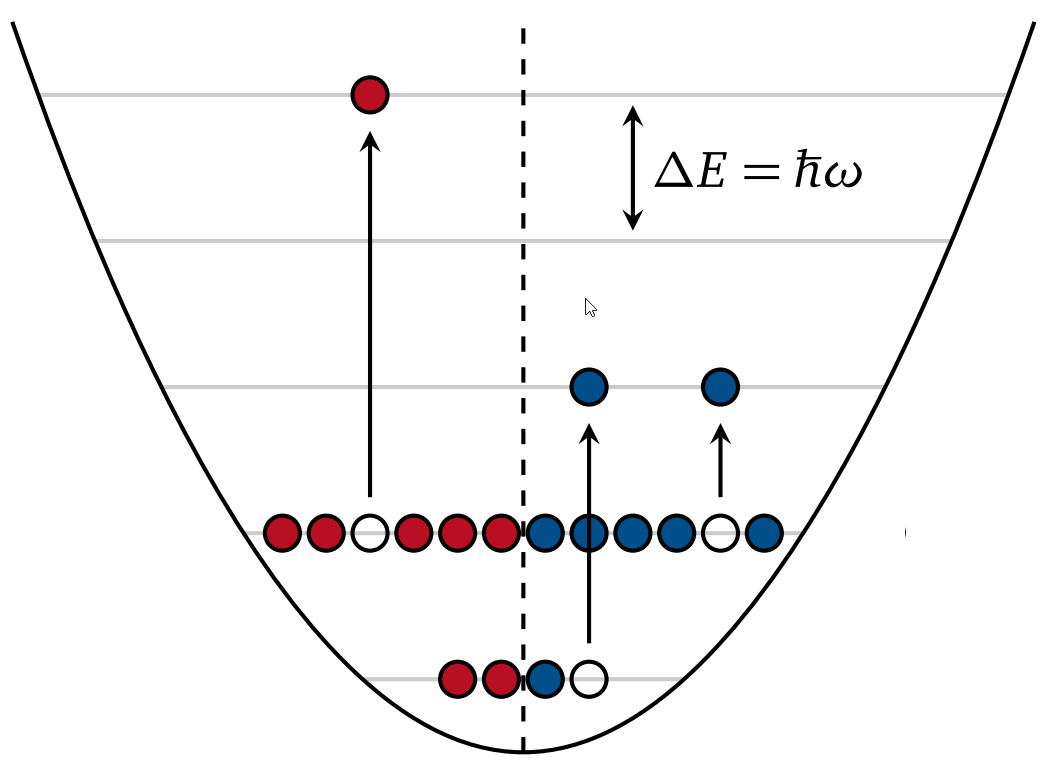
\includegraphics[width=.4\textwidth]{media/ncsm.png}
  \caption{An example configuration of \n{16}{O} with $N_\mathrm{max} = 6$ excitation quanta. The lines show the different energy levels of the harmonic oscillator. Multiple nucleons (blue and red balls) are excited from their ground state, leaving holes(uncolored balls).}
  \label{fig:ncsm}
\end{wrapfigure}
This method is still not computationally feasible, since the many-body basis is infinite dimensional. We thus have to truncate the Hilbert space $\H_A$ to a smaller model space $\mathcal{M}$ of dimension $D$. The \n{16}{O} configuration shown in \autoref{fig:ncsm} has $N_\mathrm{max} = 6$ excitation quanta and is the respective slater determinant is present in all model spaces with $N_\mathrm{max} \geq 6$. In the NCSM, this truncation is chosen such that slater determinants with at most $N_\mathrm{max}$ excitation quanta are used in the model space.
% Bild von Nmax-
To solve the eigenvalue problem in the finite model space, we have to do a variational calculation with the trial state
\begin{equation}
  \ket{\psi_T} = \sum_i^{D} C_i \ket{\psi_i},
\end{equation}
which formally leads to the matrix eigenvalue problem, truncated to the model space $\mathcal{M}$. Obviously, the reconstructed many-body state $\psi_T(D)$ and in particular the calculated energy $E_n(D)$ is dependent on the dimension $D$ of the model space. From the properties of variational principles, it follows that the ground state energy $E_0$ is always less then the expectation value of the trial state. In fact, the much stronger \textit{Hylleraas-Undheim Theorem} holds. It states that all states have a monotonously decreasing energy
\begin{equation}
  E_n(D) \geq E_n(D+1)
\end{equation}
with increasing model space dimension $D$, if the model space of dimension $D+1$ is constructed by appending one basis vector to the model space of dimension $D$. Furthermore, the energies cannot fall below the exact energy $E_n$ of the full Hilbert space. Both the monotonicity and the boundedness from below imply the convergence of $E_n(D)$ to the exact energy.

To calcluate the eigenvalues of truncated matrices, we can use iterative methods such as the \textit{Lanczos Algorithm} and obtain the lowest energy values. Since the matrix dimensions scale with the total amount of nucleons $A$, it is not feasible to calculate energies of higher-mass nuclei up to a satisfactory convergence. This opens doors to various extrapolation methods and is the direct connection to the interest of this thesis in extrapolating energy values using neural networks.

\subsection{Similarity Renormalization Group}
To improve the results of NCSM calculations and improve the convergence of the energy sequences, we can pre-diagonalize the Hamiltonian using the \textit{similarity renormalization group} (SRG). The idea is to use a unitary transformation of the Hamiltonian with a unitary operator $\hat{U}_\alpha$ to define an evolved Hamiltonian $\hat{H}_\alpha$ with
\begin{equation}
  \hat{H}_\alpha = \hat{U}_\alpha^\dagger \hat{H} \hat{U}_\alpha =: T_\mathrm{rel} + V_\alpha.
\end{equation}
The evolution of $\hat{H}_\alpha$ is given by the \textit{flow equation}
\begin{align}
  \frac{\mathrm{d}\hat{H}_\alpha}{\mathrm{d}\alpha} = [\hat{\eta}_\alpha, \hat{H}_\alpha]
\end{align}
with the \textit{evolution generator}
\begin{equation}
  \hat{\eta}_\alpha = \frac{\mathrm{d}\hat{H}_\alpha}{\mathrm{d}\alpha} \hat{U}^\dagger_\alpha = -\hat{\eta}_\alpha^\dagger.
\end{equation}
For a choice of an evolution generator and a flow parameter $\alpha$, we get an evolved Hamiltonian $\hat{H}_\alpha$ with matrix entries more focused to the diagonal. This pre-diagonlization conserves the spectrum of $\hat{H}$ and can thus be used in No-Core Shell Model calculations to gain a faster convergence.
